\subsubsection{Versionhistorik}

\begin{longtabu} to \linewidth{@{}l l l X[j]@{}}
    Version &    Dato &    Ansvarlig &    Beskrivelse\\[-1ex]
    \midrule
   
    	
\label{version_Systemark}
\end{longtabu}

\chapter{Indledning}
I dette projekt var problemstilling at lave en invasiv blodtrykmåler til en valgfri institution. Der er i den forbindelse blevet arbejdet med blodtryks-måling, udvikling af hardware til blodtryksmåleren samt udarbejdelse af et program til analyse af blodtryks-målingen.\\ 
\\
Motivationen for projektet bygger på, at der i klinisk praksis ofte er behov for kontinuert at kunne monitorerer en patients blodtryk. Dette er især vigtigt på en operationsstue, hvor blodtrykket er en vigtig parameter til monitorering af deres helbredstilstand, hvilket derfor ligger til grund for udarbejdelsen af dette projekt.\\
\begin{figure}[H]
	\centering
	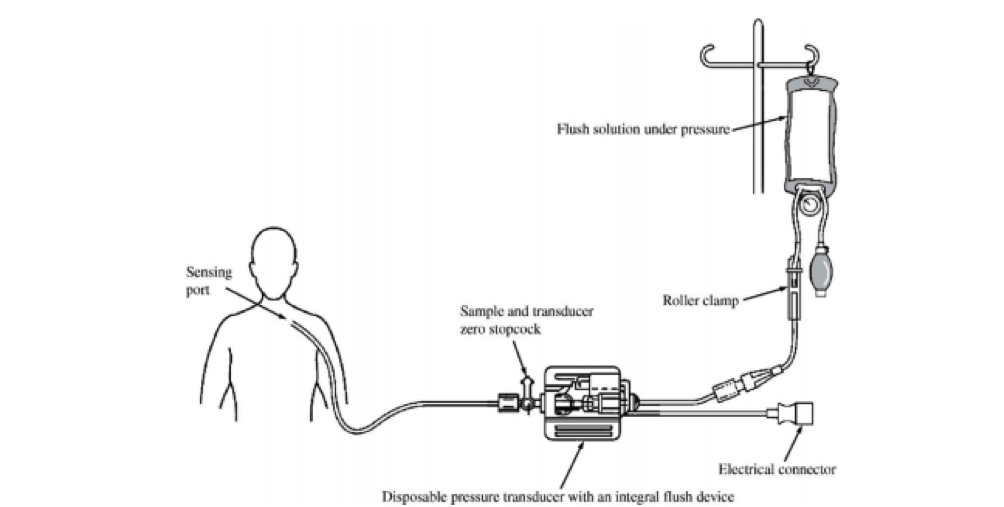
\includegraphics[width=0.8\textwidth]{Figurer/Indledning/Opstilling}
	\label{Opstilling}
	\caption{Tilslutningen af væskefyldt kateter}
\end{figure}
Da det er vigtigt med kontinuerte målinger af blodtrykket bliver målingen foretaget invasivt. På billedet ses det hvordan blodtryksmålesystemet er tilsluttet patientens arterier via et væskefyldt kateter.\\
Projektets resultat vil kunne hjælpe sundhedsfaglig personale med at bevarer overblikket over deres patients fysiske tilstand under en operation. Da det både kan være en planlagt eller akut situation på operationsstuen er det vigtigt, at systemet virker optimalt og udøver den bedste hjælp til personalet.\\
\\  
I dette projekt der skal arbejdes på at udarbejdet et system, der kan tilsluttes det væskefyldte kateter og som kan vise en blodtryks kurve, samt blodtryks værdier på en computerskærm. \\
Systemet skal bestå af to elementer:
\begin{enumerate}
	\item Det ene element består af et elektronisk kredsløb, der forstærker signalet fra transduceren og filtrerer signalet med et indbygget analogt filter.
	\item Det andet element er et program, der afbilder blodtrykket grafisk som funktion af tiden. Programmet skal lige ledes vise blodtryksværdier, samt puls og kunne udløse en alarm hvis grænseværdier for blodtrykket overskrides. 
\end{enumerate}



  
